\documentclass[11pt,a4paper]{article}

% ============ PACKAGES ============
\usepackage[utf8]{inputenc}
\usepackage[T1]{fontenc}
\usepackage{lmodern}
\usepackage[margin=1in]{geometry}
\usepackage{graphicx}
\usepackage{booktabs}
\usepackage{longtable}
\usepackage{array}
\usepackage{tabularx}
\usepackage{colortbl}
\usepackage{xcolor}
\usepackage{xurl}
\usepackage{hyperref}
\usepackage{titlesec}
\usepackage{enumitem}
\usepackage{fancyhdr}
\usepackage{float}
\usepackage{makecell}
\usepackage{tocloft}
\usepackage{caption}
\usepackage{listings}
\usepackage{multicol}
\usepackage{tcolorbox}
\usepackage{multirow}
\usepackage{microtype}
\usepackage{ragged2e}
\setlength{\emergencystretch}{3em}

% ============ HYPERREF CONFIG ============
\hypersetup{
    colorlinks=true,
    linkcolor=headerblue,
    urlcolor=headerblue!70!black,
    citecolor=accentred!70!black,
    pdftitle={Anthropic Distillation Attacks -- Adversary Profiling Using MITRE ATT\&CK},
    pdfauthor={Vishnu V},
    pdfsubject={CTI Adversary Profiling Assignment},
    pdfkeywords={MITRE ATT\&CK, Distillation, Anthropic, DeepSeek, Moonshot, MiniMax, CTI},
    breaklinks=true
}

% ============ COLOR DEFINITIONS ============
\definecolor{headerblue}{HTML}{1B3A5C}
\definecolor{lightblue}{HTML}{F0F4F8}
\definecolor{accentred}{HTML}{C0392B}
\definecolor{accentgreen}{HTML}{27AE60}
\definecolor{rowgray}{HTML}{F5F5F5}
\definecolor{tacticbg}{HTML}{E8F0FE}
\definecolor{codebg}{HTML}{F8F8F8}
\definecolor{classification}{HTML}{C0392B}

% ============ PAGE STYLE ============
\setlength{\headheight}{22pt}
\pagestyle{fancy}
\fancyhf{}
\fancyhead[L]{\small\textcolor{classification}{\textbf{TLP:CLEAR}}}
\fancyhead[R]{\small\textcolor{gray}{Anthropic Distillation Attacks -- Adversary Profile}}
\fancyfoot[C]{\thepage}
\renewcommand{\headrulewidth}{0.4pt}
\renewcommand{\headrule}{\hbox to\headwidth{\color{headerblue}\leaders\hrule height 0.8pt\hfill}}
\renewcommand{\footrulewidth}{0.2pt}
\renewcommand{\footrule}{\hbox to\headwidth{\color{gray!40}\leaders\hrule height 0.2pt\hfill}}

% ============ SECTION FORMATTING ============
\titleformat{\section}{\Large\bfseries\color{headerblue}}{\thesection}{1em}{}[\vspace{-3pt}\titlerule\vspace{3pt}]
\titleformat{\subsection}{\large\bfseries\color{headerblue!80!black}}{\thesubsection}{1em}{}
\titleformat{\subsubsection}{\normalsize\bfseries\color{headerblue!60!black}}{\thesubsubsection}{1em}{}

% ============ TOC FORMATTING ============
\renewcommand{\cftsecfont}{\bfseries\color{headerblue}}
\renewcommand{\cftsecpagefont}{\bfseries}
\renewcommand{\cftsecleader}{\cftdotfill{\cftsecdotsep}}
\renewcommand{\cftsecdotsep}{\cftdot}
\setlength{\cftbeforetoctitleskip}{0pt}
\renewcommand{\cfttoctitlefont}{\huge\bfseries\color{headerblue}}

% ============ LISTINGS (JSON CODE BLOCK) ============
\lstdefinestyle{jsonstyle}{
    backgroundcolor=\color{codebg},
    basicstyle=\ttfamily\scriptsize,
    breaklines=true,
    frame=single,
    rulecolor=\color{gray!50},
    showstringspaces=false,
    tabsize=2,
    language=json,
    keywordstyle=\color{blue},
    stringstyle=\color{accentgreen},
    commentstyle=\color{gray}
}

% ============ TABLE HELPERS ============
\newcolumntype{L}[1]{>{\raggedright\arraybackslash}p{#1}}
\newcolumntype{C}[1]{>{\centering\arraybackslash}p{#1}}

% ============ TITLE PAGE INFO ============
\title{}
\author{}
\date{}

% ============ DOCUMENT BEGINS ============
\begin{document}

% ============ TITLE PAGE ============
\begin{titlepage}
\thispagestyle{empty}
\centering

% Top classification bar
\begin{tcolorbox}[colback=classification, colframe=classification, boxrule=0pt, arc=0pt, outer arc=0pt, width=\textwidth, left=8pt, right=8pt, top=6pt, bottom=6pt]
{\color{white}\bfseries\Large TLP:CLEAR -- PUBLIC RELEASE}
\end{tcolorbox}
\vspace{2cm}

% Main title block
\begin{tcolorbox}[colback=lightblue, colframe=headerblue, boxrule=1.5pt, arc=2pt, sharp corners=south, width=\textwidth-2cm, left=16pt, right=16pt, top=16pt, bottom=16pt]
\centering
{\LARGE\bfseries\color{headerblue} Adversary Profiling Using\\ MITRE ATT\&CK}\\[6pt]
{\large\color{gray!60!black} Provider-Reported Campaign Case Study}\\[12pt]
\rule{0.6\textwidth}{1pt}\\[10pt]
{\Large\bfseries\color{accentred} Anthropic Distillation Attacks\\ by Chinese AI Labs (2026)}\\[6pt]
{\normalsize\color{gray!60!black} A Structured Cyber Threat Intelligence Adversary Profile Report}
\end{tcolorbox}

\vspace{1.5cm}

% Author block
\begin{minipage}{0.55\textwidth}
\centering
\large
\textbf{Vishnu V}\\
Software Engineer / ML Engineer\\
\vspace{4pt}
\small\textit{CTI Adversary Profiling Assignment}\\
\small July 11, 2026
\end{minipage}

\vfill

% Bottom classification bar
\begin{tcolorbox}[colback=classification, colframe=classification, boxrule=0pt, arc=0pt, outer arc=0pt, width=\textwidth, left=8pt, right=8pt, top=6pt, bottom=6pt]
{\color{white}\bfseries\Large TLP:CLEAR -- PUBLIC RELEASE}
\end{tcolorbox}

\end{titlepage}

% ============ TABLE OF CONTENTS ============
\newpage
\tableofcontents
\newpage

% ============================================================
% SECTION 1: EXECUTIVE SUMMARY
% ============================================================
\section{Executive Summary}

In February 2026, Anthropic reported that accounts linked by its investigators to DeepSeek, Moonshot AI, and MiniMax conducted industrial-scale model-distillation campaigns against Claude, generating more than 16 million exchanges through about 24,000 accounts that Anthropic characterized as fraudulent \cite{anthropic_blog}\cite{techcrunch}. The activity allegedly used legitimate API functionality at abnormal scale to collect outputs covering agentic reasoning, tool use, and coding for training competing models \cite{anthropic_blog}\cite{engadget}. In June 2026, Anthropic separately accused operators affiliated with Alibaba's Qwen lab of generating 28.8 million interactions through nearly 25,000 accounts \cite{reuters_alibaba}\cite{forbes_distillation}. These are serious, well-sourced provider allegations, but the underlying telemetry and attribution evidence are not public; this report therefore distinguishes Anthropic's confidence assessment from independent verification.

The dispute broadened in July 2026 when Reuters reported that Alibaba restricted internal use of Claude Code and that China's National Vulnerability Database issued a warning about China-focused checks in the tool \cite{indiatoday_alibaba}\cite{scmp_claudecode}. Those later events provide geopolitical context; they do not independently validate Anthropic's attribution of the earlier distillation campaigns.

\begin{tcolorbox}[colback=lightblue, colframe=headerblue, boxrule=1pt, arc=2pt, sharp corners=south, title=\textbf{Key Facts at a Glance}]
\begin{itemize}[leftmargin=20pt, noitemsep, nosep]
    \item \textbf{Target:} Anthropic (Claude AI Model Platform)
    \item \textbf{Threat Actors:} DeepSeek, Moonshot AI, MiniMax (Feb 2026); Alibaba/Qwen (Jun 2026)
    \item \textbf{Attack Vector:} API abuse via $\sim$24,000 fraudulent accounts through proxy services
    \item \textbf{Scale:} 16M+ exchanges (Feb 2026); 28.8M exchanges (Jun 2026, Alibaba)
    \item \textbf{Assessed Impact:} Potential replication of proprietary model capabilities and erosion of safety controls
    \item \textbf{Attribution Confidence:} High according to Anthropic; independently unverified from public evidence
\end{itemize}
\end{tcolorbox}

\newpage

% ============================================================
% SECTION 2: ADVERSARY OVERVIEW
% ============================================================
\section{Adversary Overview}

\subsection{Attributed Entity: DeepSeek}

\begin{table}[H]
\centering
\renewcommand{\arraystretch}{1.3}
\begin{tabularx}{\textwidth}{|L{4.5cm}|X|}
\hline
\rowcolor{headerblue}
\textcolor{white}{\textbf{Attribute}} & \textcolor{white}{\textbf{Detail}} \\
\hline
Group Name & DeepSeek (Shen Du Qiu Suo) \\
\hline
Aliases & DeepSeek AI, Hangzhou DeepSeek Artificial Intelligence Co., Ltd. \\
\hline
Organizational Context & Hangzhou-based AI company associated with High-Flyer Capital Management. The public evidence reviewed here does not establish state direction of the reported activity. \\
\hline
Known Targets & US frontier AI models (Anthropic Claude, OpenAI GPT); targeted reasoning capabilities, reward modeling, censorship-safe query rewrites \\
\hline
Campaign Scale & 150,000+ exchanges through fraudulent accounts \cite{anthropic_blog} \\
\hline
Sophistication Level & High, employing chain-of-thought elicitation techniques to generate structured training data; synchronized traffic across accounts with coordinated timing and shared payment methods \cite{anthropic_blog}\cite{treblle} \\
\hline
Prior Campaigns & DeepSeek-R1 model release (January 2025) disrupted global AI markets; OpenAI accused DeepSeek of distillation against GPT models the same week as Anthropic's disclosure \cite{reuters_alibaba}\cite{linkedin_keltner} \\
\hline
\end{tabularx}
\caption{DeepSeek Threat Group Profile}
\label{tab:deepseek}
\end{table}

\subsection{Attributed Entity: Moonshot AI}

\begin{table}[H]
\centering
\renewcommand{\arraystretch}{1.3}
\begin{tabularx}{\textwidth}{|L{4.5cm}|X|}
\hline
\rowcolor{headerblue}
\textcolor{white}{\textbf{Attribute}} & \textcolor{white}{\textbf{Detail}} \\
\hline
Group Name & Moonshot AI (Yue Zhi An Mian) \\
\hline
Aliases & Moonshot, Kimi AI \\
\hline
Organizational Context & Beijing-based, venture-backed AI company. The public evidence reviewed here does not establish state direction of the reported activity. \\
\hline
Known Targets & Anthropic Claude API; targeted agentic reasoning, tool use, coding, data analysis, computer-use agent development, computer vision, and reasoning trace reconstruction \\
\hline
Campaign Scale & 3,400,000+ exchanges across hundreds of fraudulent accounts spanning multiple access pathways \cite{anthropic_blog}\cite{techcrunch} \\
\hline
Sophistication Level & High, varying account types to evade detection as a coordinated operation; used later-phase targeted approach to extract and reconstruct Claude's reasoning traces; request metadata matched public profiles of senior Moonshot staff \cite{anthropic_blog} \\
\hline
\end{tabularx}
\caption{Moonshot AI Threat Group Profile}
\label{tab:moonshot}
\end{table}

\subsection{Attributed Entity: MiniMax}

\begin{table}[H]
\centering
\renewcommand{\arraystretch}{1.3}
\begin{tabularx}{\textwidth}{|L{4.5cm}|X|}
\hline
\rowcolor{headerblue}
\textcolor{white}{\textbf{Attribute}} & \textcolor{white}{\textbf{Detail}} \\
\hline
Group Name & MiniMax (Xi Yu Ke Ji) \\
\hline
Aliases & MiniMax AI, listed on Hong Kong Stock Exchange (0100.HK) \cite{reuters_alibaba} \\
\hline
Organizational Context & Shanghai-based AI company with a public market listing. The public evidence reviewed here does not establish state direction of the reported activity. \\
\hline
Known Targets & Anthropic Claude API; targeted agentic coding, tool use and orchestration; pivoted to target Claude's latest model within 24 hours of release \\
\hline
Campaign Scale & 13,000,000+ exchanges, the largest of the three campaigns \cite{anthropic_blog}\cite{techcrunch} \\
\hline
Sophistication Level & Very high according to Anthropic, which reported detection during an active campaign and a rapid traffic shift after a Claude model release \cite{anthropic_blog}\cite{treblle} \\
\hline
\end{tabularx}
\caption{MiniMax Threat Group Profile}
\label{tab:minimax}
\end{table}

\begin{figure}[H]
    \centering
    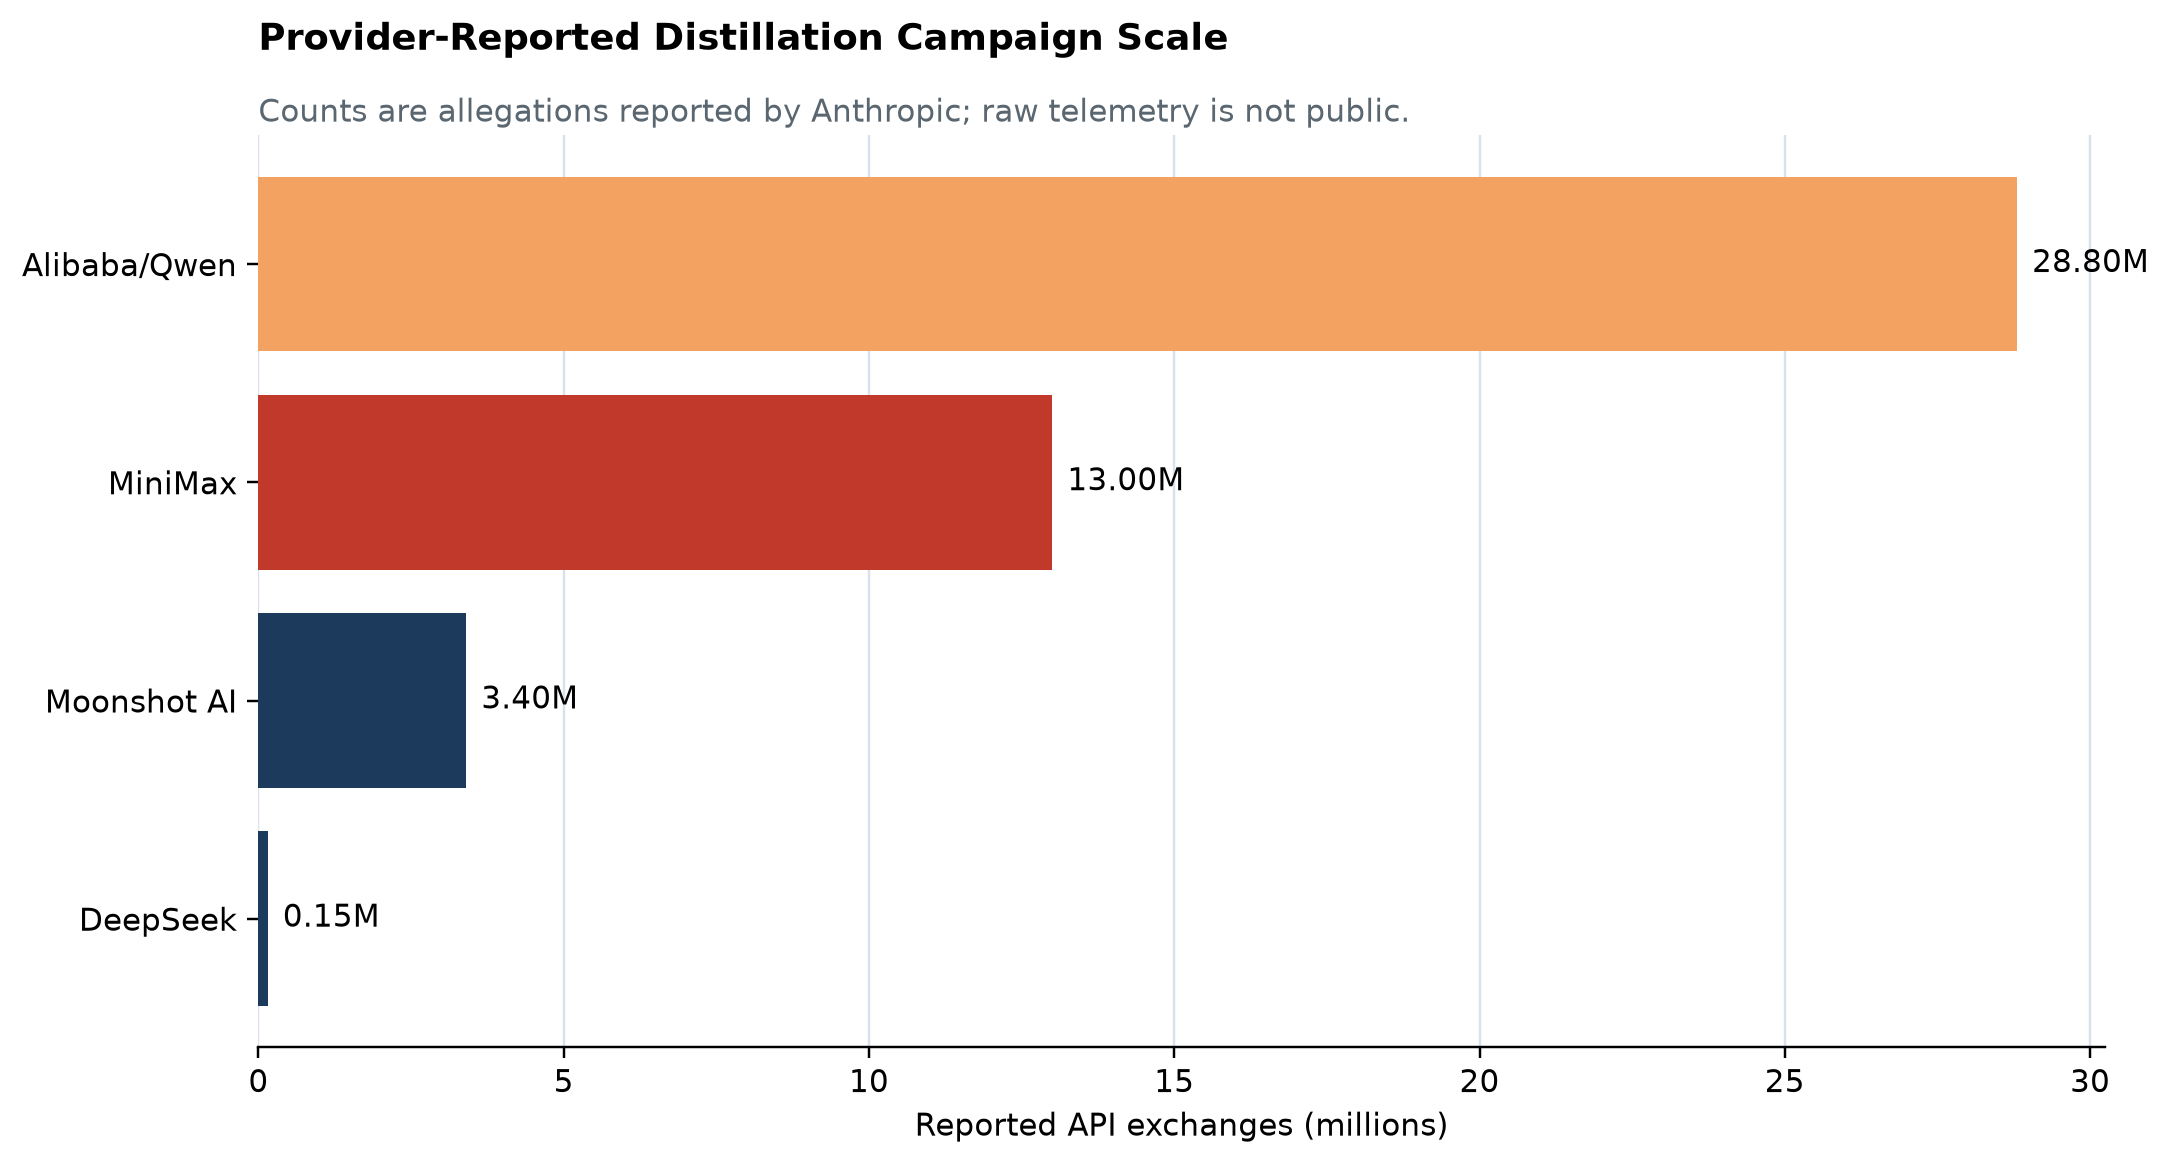
\includegraphics[width=0.85\textwidth]{distillation_attack_scale.png}
    \caption{Distillation Attack Scale (Number of API Exchanges by Threat Group)}
    \label{fig:attack_scale}
\end{figure}

\subsection{Collective Motivation}

Anthropic assessed the likely motivation as \textbf{economic and strategic competitive advantage}: reducing the cost and time required to reproduce frontier-model capabilities \cite{anthropic_blog}\cite{mashable}. US officials have separately framed industrial-scale distillation as an intellectual-property and national-security concern \cite{forbes_distillation}. Public reporting does not establish direct state sponsorship of the named campaigns.

\newpage

% ============================================================
% SECTION 3: ATTACK TIMELINE
% ============================================================
\section{Attack Timeline}

\subsection{Pre-Attack Phase}

\begin{itemize}[leftmargin=20pt, noitemsep]
    \item \textbf{Ongoing (pre-2026):} Anthropic restricts commercial Claude access in China for national security reasons, requiring all users to verify account authenticity and geographic location \cite{anthropic_blog}.
    \item \textbf{Reconnaissance:} The labs research Claude's capabilities, API structure, rate limits, account verification processes, and model release schedules. MiniMax monitors Anthropic's public product roadmap to time their extraction campaigns \cite{anthropic_blog}.
    \item \textbf{Infrastructure Development:} The labs establish relationships with commercial proxy services that resell access to Claude and other frontier AI models. These proxy services deploy ``hydra cluster'' architectures (sprawling networks) of fraudulent accounts distributed across the API and third-party cloud platforms. In one documented case, a single proxy network managed more than 20,000 fraudulent accounts at the same time \cite{anthropic_blog}.
\end{itemize}

\subsection{Active Attack Phase}

\begin{itemize}[leftmargin=20pt, noitemsep]
    \item \textbf{Account Creation \& Infrastructure Setup:} The labs create about 24,000 fraudulent accounts through commercial proxy services, often exploiting educational accounts, security research programs, and startup organization pathways, the verification processes most vulnerable to abuse \cite{anthropic_blog}\cite{engadget}.
    \item \textbf{DeepSeek Campaign (timing undisclosed):} DeepSeek generated 150,000+ synchronized exchanges. DeepSeek coordinates traffic across accounts with identical patterns, shared payment methods, and load-balancing timing. DeepSeek engineers prompts to elicit chain-of-thought reasoning, asking Claude to ``imagine and articulate the internal reasoning behind a completed response and write it out step by step.'' Additional prompts target censorship-safe rewrites of sensitive queries about dissidents, party leaders, and authoritarianism \cite{anthropic_blog}.
    \item \textbf{Moonshot AI Campaign (timing undisclosed):} Moonshot generated 3,400,000+ exchanges across hundreds of varied account types spanning multiple access pathways. Initial phase targets agentic reasoning, tool use, coding, data analysis, and computer vision. A later phase shifts to a more targeted approach attempting to extract and reconstruct Claude's reasoning traces \cite{anthropic_blog}.
    \item \textbf{MiniMax Campaign (active, detected mid-operation):} MiniMax generated 13,000,000+ exchanges targeting agentic coding and tool use orchestration. Anthropic detects the campaign while still active, before MiniMax releases the model it was training. When Anthropic releases a new Claude model mid-campaign, MiniMax pivots within 24 hours, redirecting half their traffic to the latest system \cite{anthropic_blog}\cite{treblle}.
    \item \textbf{Traffic Obfuscation:} All three labs mix distillation-focused queries with unrelated, mundane customer requests within proxy networks to flatten anomalous signals. Account types are varied to prevent the campaigns from appearing as coordinated operations \cite{anthropic_blog}\cite{treblle}.
\end{itemize}

\subsection{Detection \& Disclosure Phase}

\begin{itemize}[leftmargin=20pt, noitemsep]
    \item \textbf{Detection:} Anthropic's behavioral fingerprinting systems, cross-account correlation analysis, IP/metadata correlation, and payment metadata analysis identify the coordinated campaigns. Anthropic attributed each campaign to a specific lab with high confidence \cite{anthropic_blog}\cite{engadget}.
    \item \textbf{Industry Corroboration:} Anthropic corroborated findings with other AI labs (including OpenAI) that observed identical actors and behaviors on their own platforms \cite{anthropic_blog}\cite{cnbc}.
    \item \textbf{February 22--23, 2026:} Anthropic published its blog post ``Detecting and Preventing Distillation Attacks,'' naming DeepSeek, Moonshot AI, and MiniMax \cite{anthropic_blog}.
    \item \textbf{April 2026:} The White House OSTP accuses China-based entities of running industrial-scale distillation campaigns against US frontier models, describing the activity as theft of American AI intellectual property \cite{forbes_distillation}.
    \item \textbf{June 2026:} Anthropic sends a letter to Capitol Hill accusing Alibaba's Qwen AI lab of the largest known distillation attack to date (28.8 million) interactions through $\sim$25,000 counterfeit accounts (April 22--June 5, 2026) \cite{reuters_alibaba}\cite{forbes_distillation}.
    \item \textbf{Late June 2026:} Security researchers discover that Claude Code versions 2.1.91 through 2.1.196 contain hidden code that checks system time zones and network proxy configurations against a list of Chinese corporate and AI lab domains. When a match is found, the software embeds markers in system prompts to notify Anthropic \cite{scmp_claudecode}.
    \item \textbf{Early July 2026:} An Anthropic engineer describes the mechanism as an ``experimental'' anti-abuse feature launched in March 2026 to prevent unauthorized account sales and distillation. Anthropic removes the code \cite{scmp_claudecode}.
    \item \textbf{July 2026:} China's National Vulnerability Database (NVDB), overseen by the Ministry of Industry and Information Technology, issued a formal security alert labeling the tracking mechanism a ``serious threat'' and a ``back-door vulnerability.'' The regulator advises organizations to uninstall or upgrade \cite{scmp_claudecode}.
    \item \textbf{July 2026:} Reuters reports that Alibaba restricted internal use of Claude Code and directed employees toward an internal alternative \cite{indiatoday_alibaba}.
\end{itemize}

\newpage

% ============================================================
% SECTION 4: ATT&CK TECHNIQUE MAP
% ============================================================
\section{ATT\&CK Technique Map}

MITRE ATT\&CK models activity against enterprise systems, while this case concerns abuse of an AI service. The table below therefore presents a \textbf{constrained analytical analogy}, not a claim that MITRE or Anthropic assigned these techniques. Only mappings with a defensible semantic relationship are retained. AI-native behavior is mapped separately to MITRE ATLAS.

\small
\begin{longtable}{|p{2.5cm}|p{1.8cm}|p{3.2cm}|p{6.8cm}|}
\hline
\rowcolor{headerblue}
\textcolor{white}{\textbf{ATT\&CK Tactic}} & \textcolor{white}{\textbf{Technique ID}} & \textcolor{white}{\textbf{Technique Name}} & \textcolor{white}{\textbf{Evidence and Mapping Confidence}} \\
\hline
\endfirsthead

\hline
\rowcolor{headerblue}
\textcolor{white}{\textbf{ATT\&CK Tactic}} & \textcolor{white}{\textbf{Technique ID}} & \textcolor{white}{\textbf{Technique Name}} & \textcolor{white}{\textbf{Evidence and Mapping Confidence}} \\
\hline
\endhead

\hline
\multicolumn{4}{|r|}{\small\itshape Continued on next page} \\
\hline
\endfoot

\hline
\endlastfoot

Resource Development & T1583.006 & Acquire Infrastructure: Web Services & Anthropic reported use of commercial proxy services. \textbf{Medium confidence analogy}: the service was acquired for operational access, although it was not conventional C2 infrastructure \cite{anthropic_blog}. \\
\rowcolor{rowgray}
Persistence & T1136.003 & Create Account: Cloud Account & Anthropic reported large-scale creation of service accounts. \textbf{High confidence analogy}: SaaS account creation is semantically closer than the previously used Local Account sub-technique \cite{anthropic_blog}. \\
Initial Access & T1078.004 & Valid Accounts: Cloud Accounts & Requests authenticated through functioning accounts and API credentials. \textbf{Medium confidence analogy}: credentials were allegedly obtained through fraudulent enrollment, not compromise of an existing victim tenant \cite{anthropic_blog}. \\
\rowcolor{rowgray}
Command and Control & T1090.002 & Proxy: External Proxy & Commercial proxies obscured the origin and coordinated traffic. \textbf{Low confidence analogy}: ATT\&CK defines this within C2, whereas this case involved access mediation to a legitimate AI service \cite{anthropic_blog}. \\
Exfiltration & T1029 & Automated Exfiltration & The reported campaign automated output retrieval at very large scale. \textbf{Low confidence analogy}: no enterprise host compromise or conventional exfiltration path was publicly demonstrated \cite{anthropic_blog}. \\

\caption{Constrained MITRE ATT\&CK Analogies for the Reported Campaigns}
\label{tab:attack_map}
\end{longtable}

\subsection{ATT\&CK Navigator Layer}

The retained layer contains \textbf{five techniques across five tactics}:

\begin{enumerate}[leftmargin=20pt, noitemsep]
    \item Resource Development (T1583.006)
    \item Persistence (T1136.003)
    \item Initial Access (T1078.004)
    \item Command and Control (T1090.002)
    \item Exfiltration (T1029)
\end{enumerate}

\noindent\textbf{Note:} The accompanying Navigator layer records confidence and caveats in each technique comment. It should be read as an analyst-created crosswalk, not an official MITRE or Anthropic mapping.

\begin{figure}[H]
    \centering
    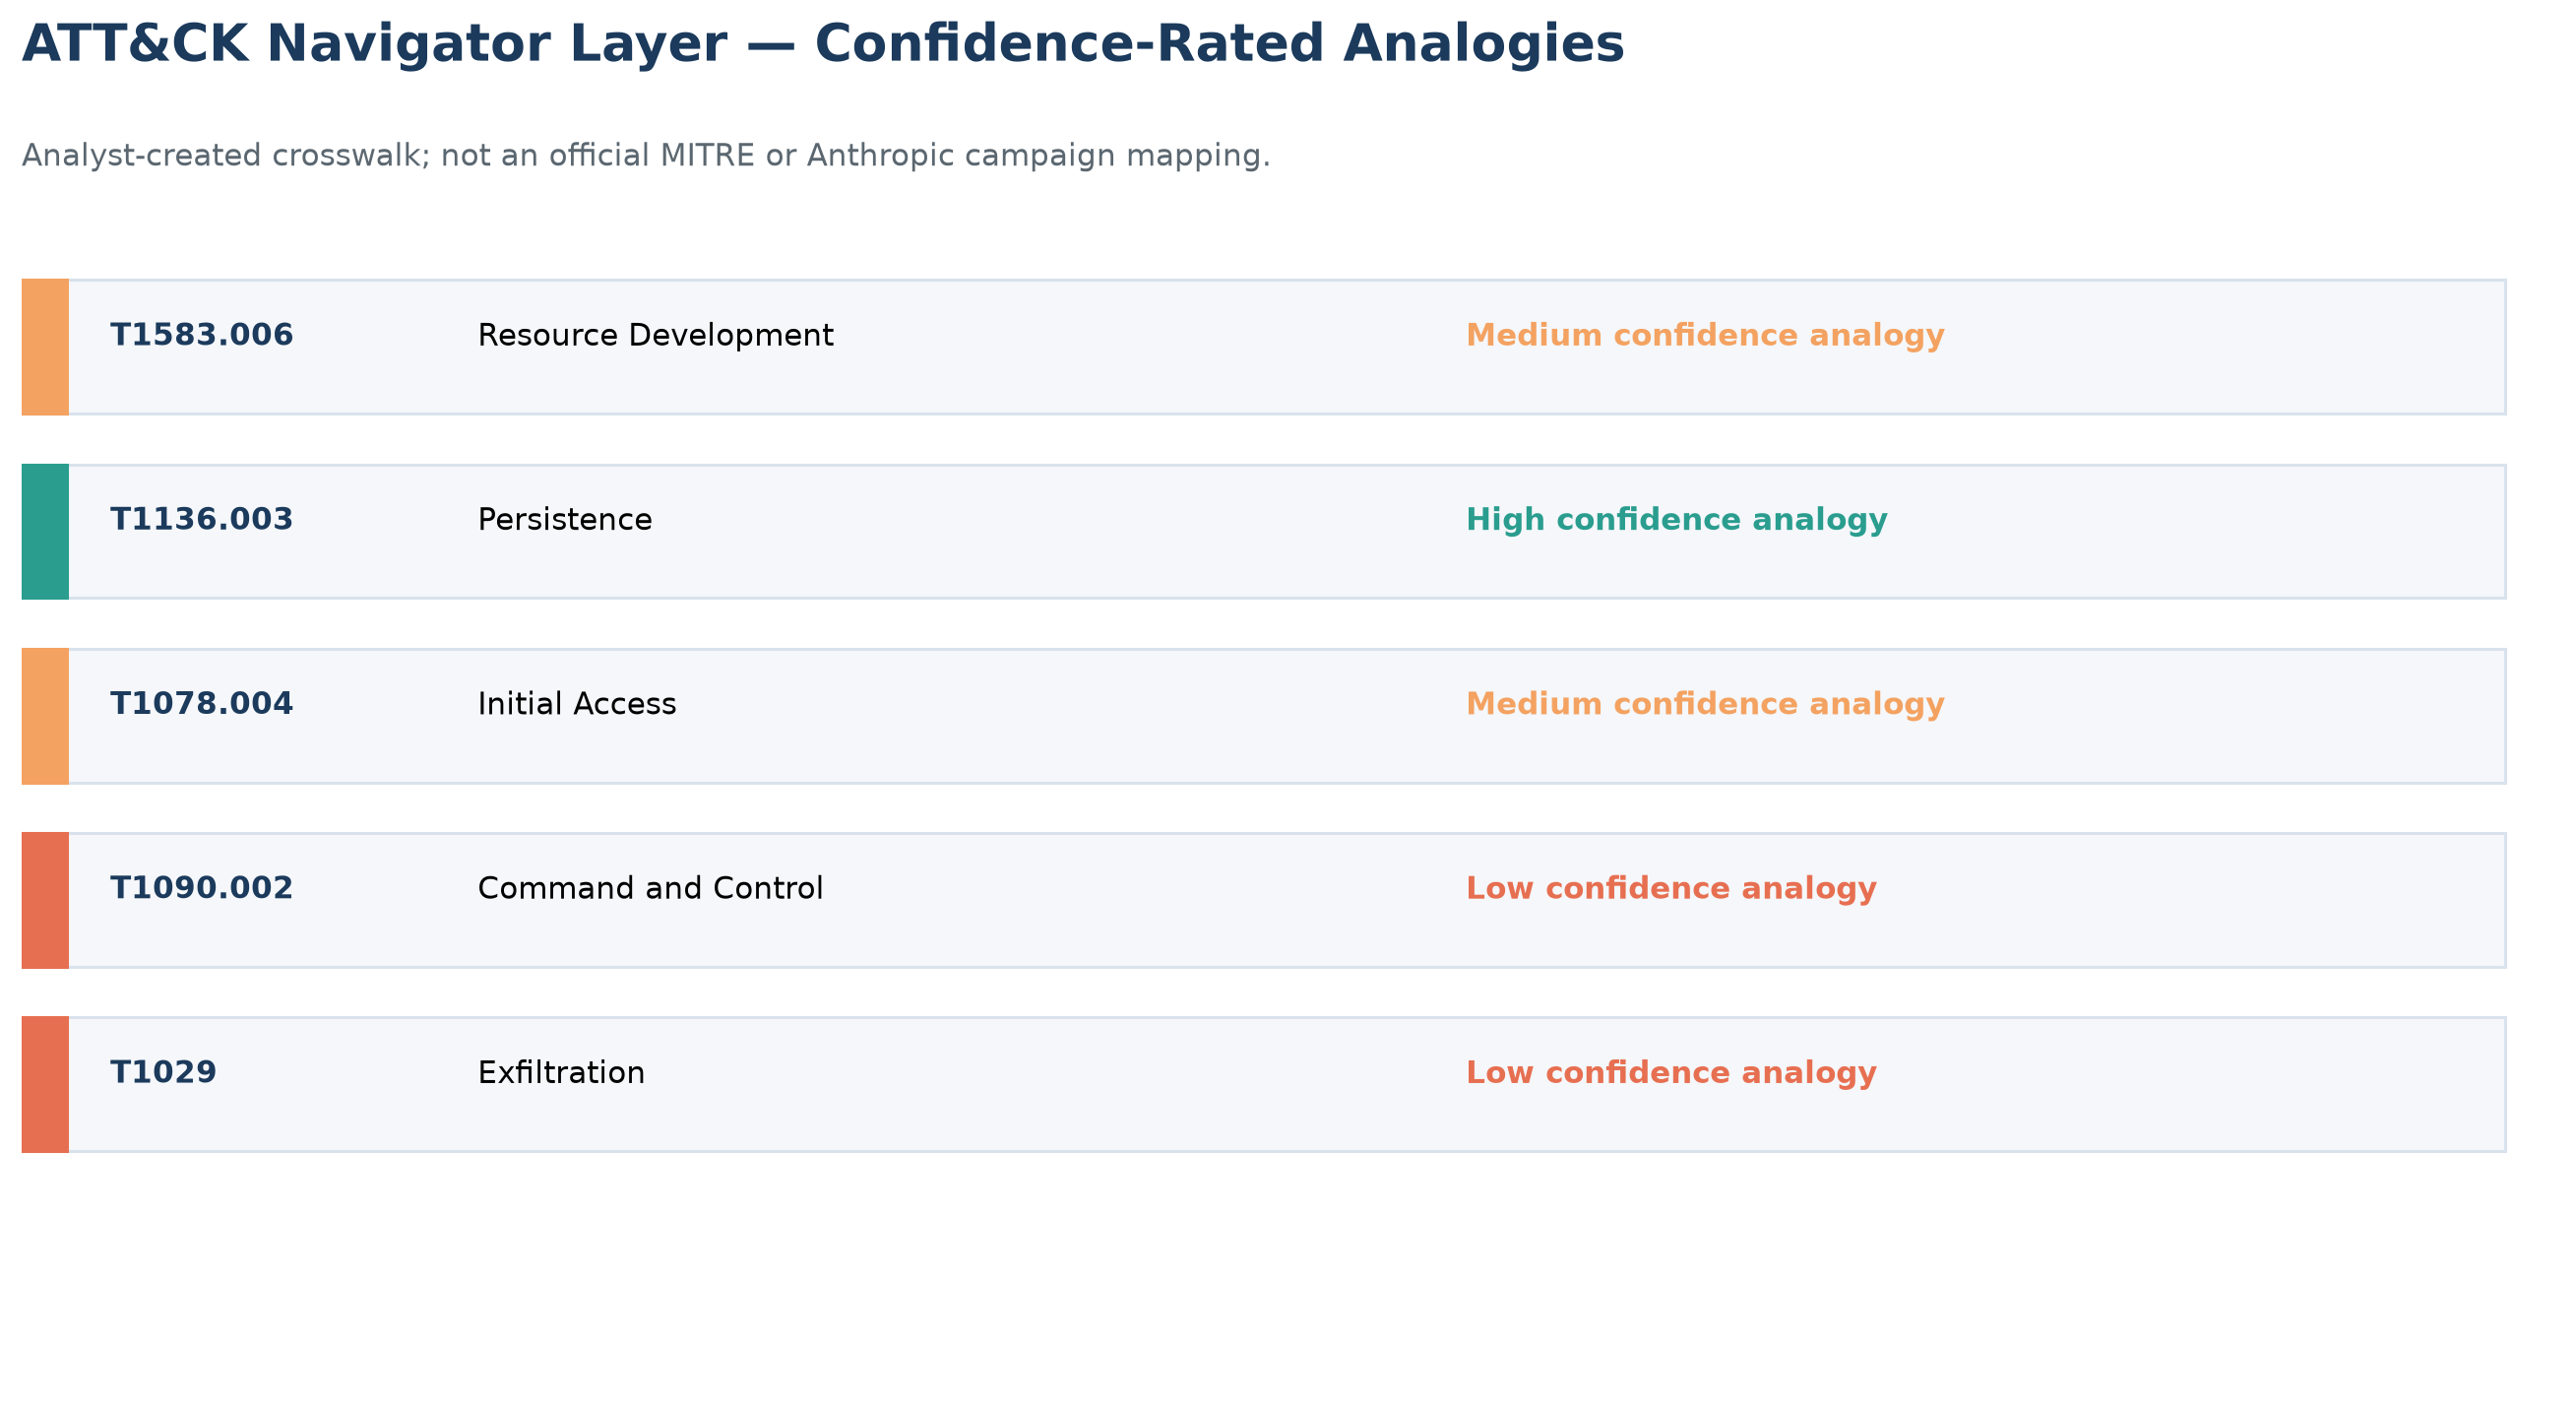
\includegraphics[width=\textwidth]{distillation_attack_navigator.png}
    \caption{MITRE ATT\&CK Navigator Layer Mapping (Tactics and Techniques Highlighted)}
    \label{fig:attack_navigator}
\end{figure}

\subsection{MITRE ATLAS Crosswalk}

MITRE ATLAS is the better semantic fit because it explicitly models adversarial activity against AI systems. The following crosswalk describes reported behavior without implying that MITRE has attributed this campaign.

\begin{table}[H]
\centering
\small
\renewcommand{\arraystretch}{1.18}
\begin{tabularx}{\textwidth}{|L{2.3cm}|L{4.1cm}|X|}
\hline
\rowcolor{headerblue}
\textcolor{white}{\textbf{ATLAS ID}} & \textcolor{white}{\textbf{Technique}} & \textcolor{white}{\textbf{Reported Behavior}} \\
\hline
AML.T0021 & Establish Accounts & Large-scale creation of allegedly fraudulent service accounts. \\
\rowcolor{rowgray}
AML.T0012 & Valid Accounts & Use of authenticated accounts and functioning API credentials. \\
AML.T0040 & AI Model Inference API Access & Repeated access to Claude through inference interfaces. \\
\rowcolor{rowgray}
AML.T0063 & Discover AI Model Outputs & Capability-focused probing and comparison of model outputs. \\
AML.T0005 & Create Proxy AI Model & Reported use of collected outputs to train models that imitate target capabilities. \\
\rowcolor{rowgray}
AML.T0024 & Exfiltration via AI Inference API & Collection of model responses through the same inference interface used for access. \\
\hline
\end{tabularx}
\caption{Analyst Crosswalk to MITRE ATLAS}
\label{tab:atlas_map}
\end{table}

\begin{figure}[H]
    \centering
    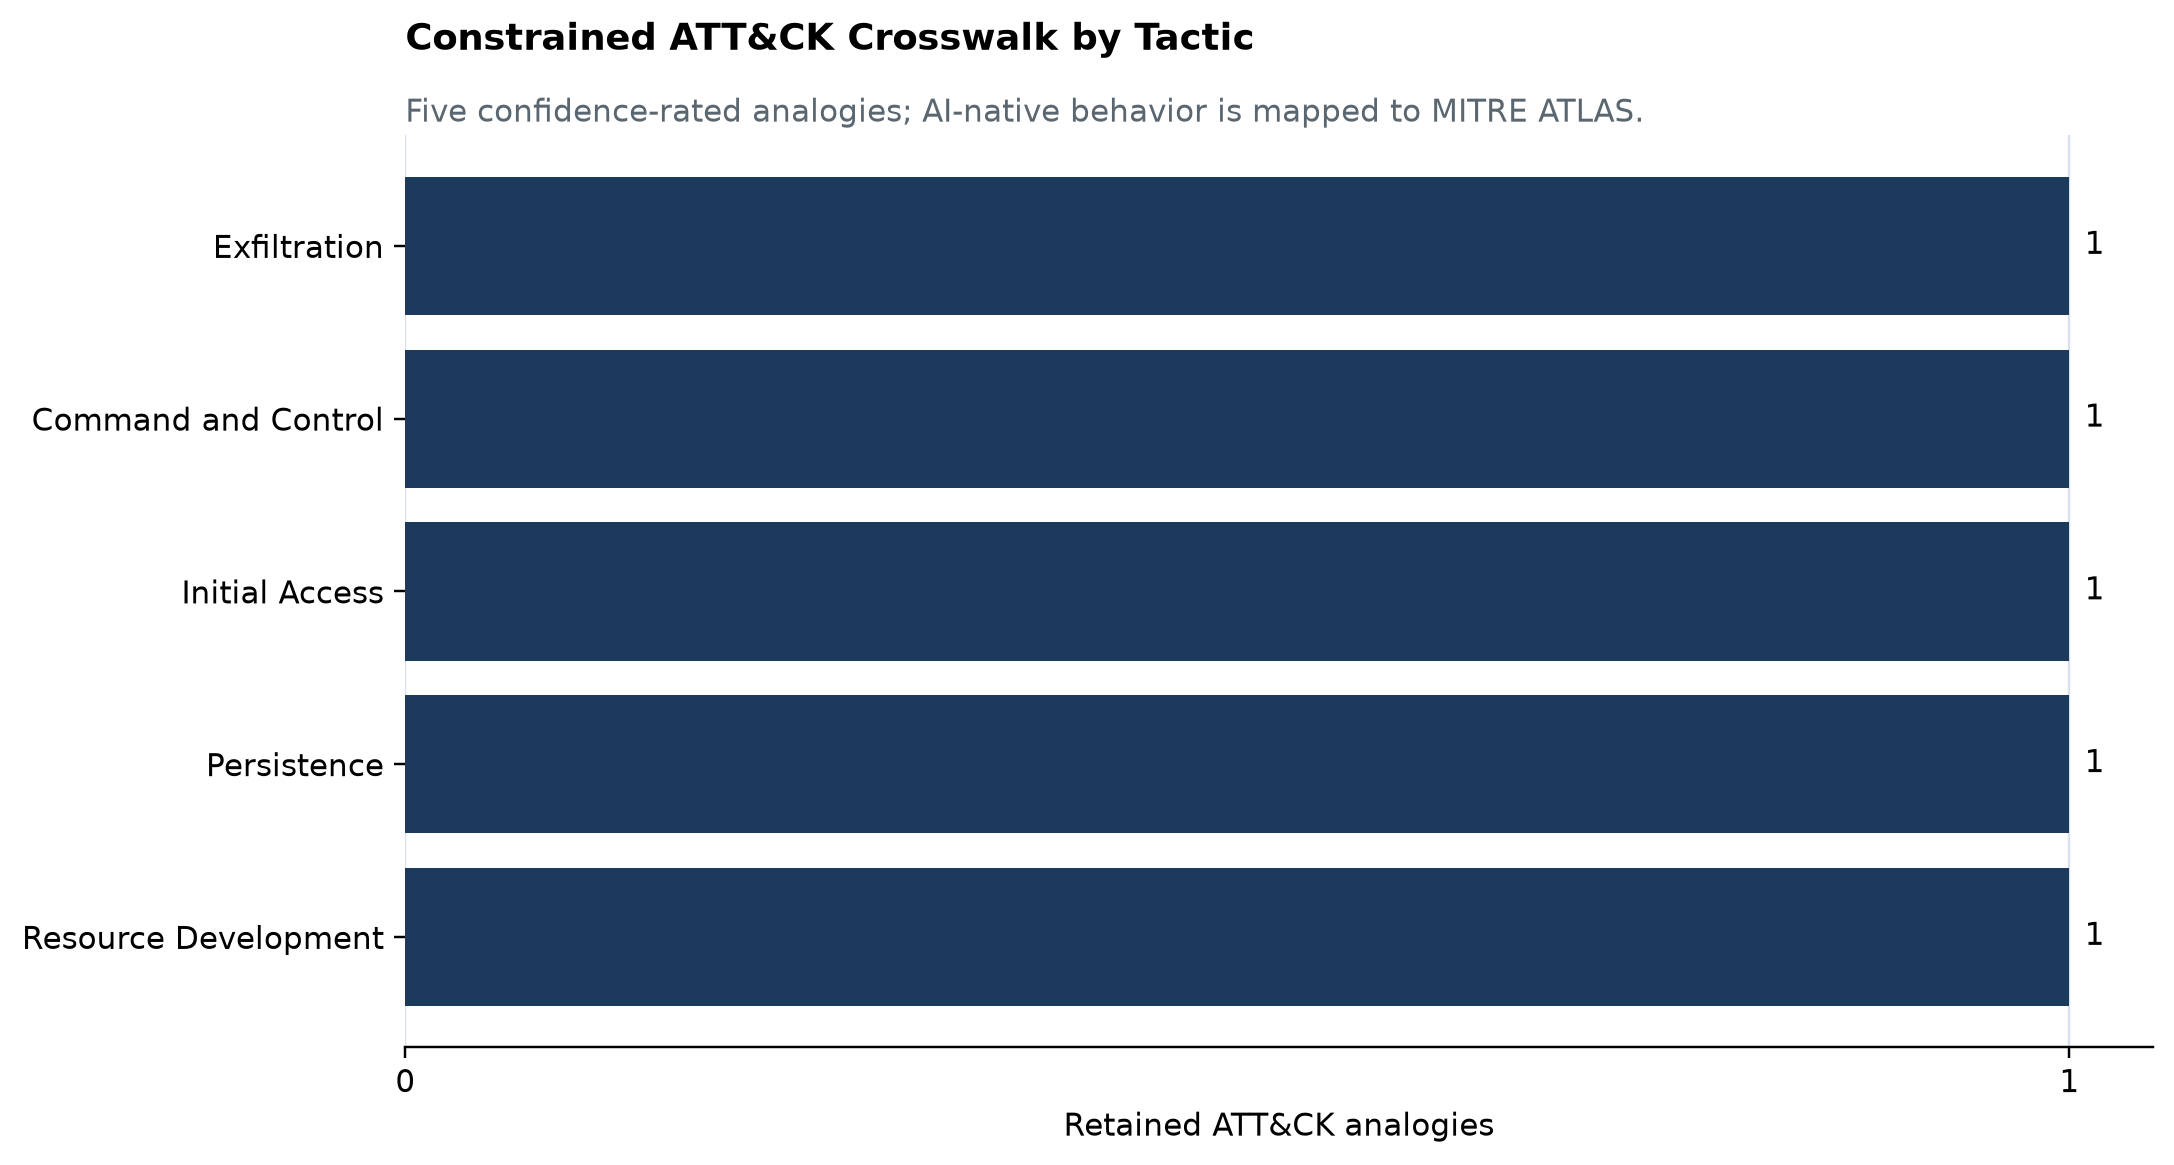
\includegraphics[width=0.9\textwidth]{attack_technique_distribution.png}
    \caption{Distribution of Retained ATT\&CK Analogies by Tactic}
    \label{fig:technique_distribution}
\end{figure}

\newpage

% ============================================================
% SECTION 5: ASSETS TARGETED
% ============================================================
\section{Assets Targeted}

\subsection{Primary Assets: Claude's Differentiated AI Capabilities}

\begin{table}[H]
\centering
\small
\renewcommand{\arraystretch}{1.2}
\begin{tabularx}{\textwidth}{|L{3.2cm}|X|L{2.5cm}|}
\hline
\rowcolor{headerblue}
\textcolor{white}{\textbf{Asset}} & \textcolor{white}{\textbf{Why It Matters}} & \textcolor{white}{\textbf{Targeted By}} \\
\hline
Agentic Reasoning & Claude's ability to plan and complete multi-step tasks. Anthropic alleged that repeated output collection could transfer parts of this capability to competing models at substantially lower development cost \cite{anthropic_blog}\cite{treblle}. & MiniMax, Moonshot AI \\
\rowcolor{rowgray}
Tool Use \& Orchestration & Claude's capacity to use external tools (code execution, API calls, web browsing) and orchestrate complex workflows, a key differentiator from competing models that enables real-world AI agent deployment \cite{anthropic_blog}. & MiniMax, Moonshot AI \\
Coding Capabilities & Claude's advanced code generation, debugging, and software engineering abilities, among the strongest in the industry and a primary commercial selling point \cite{anthropic_blog}. & MiniMax, Moonshot AI \\
\rowcolor{rowgray}
Chain-of-Thought Reasoning Data & The internal step-by-step reasoning process , which is critical for training student models to not just produce correct answers but to reason like a frontier model. DeepSeek engineered prompts to elicit this \cite{anthropic_blog}. & DeepSeek \\
Reward Model / Rubric-Based Grading & Claude's ability to function as a reward model for reinforcement learning, by using Claude to grade tasks, adversaries can bootstrap their own RL pipelines without developing independent reward models \cite{anthropic_blog}. & DeepSeek \\
\rowcolor{rowgray}
Censorship-Safe Query Rewrites & Claude's ability to rephrase queries (about dissidents, party leaders, authoritarianism) in ways that , used to train Chinese models to steer conversations away from censored topics while maintaining safety filters \cite{anthropic_blog}. & DeepSeek \\
Computer Vision \& Computer-Use Agent & Claude's capabilities in visual understanding and , which are frontier capabilities critical for building AI agents that can operate desktop environments \cite{anthropic_blog}. & Moonshot AI \\
\rowcolor{rowgray}
Reasoning Traces & The underlying reasoning structures within Claude's responses that Moonshot attempted to ``, revealing proprietary architectural knowledge about how the model reasons \cite{anthropic_blog}. & Moonshot AI \\
\hline
\end{tabularx}
\caption{Primary Assets Targeted in the Distillation Attacks}
\label{tab:assets}
\end{table}

\subsection{Secondary Assets}

\begin{table}[H]
\centering
\renewcommand{\arraystretch}{1.3}
\begin{tabularx}{\textwidth}{|L{4cm}|X|}
\hline
\rowcolor{headerblue}
\textcolor{white}{\textbf{Asset}} & \textcolor{white}{\textbf{Impact}} \\
\hline
API Infrastructure & $\sim$24,000 fraudulent accounts consumed API resources, degrading service quality for legitimate customers and imposing infrastructure costs \cite{anthropic_blog}. \\
\rowcolor{rowgray}
Safety Safeguards & Distilled models strip away Anthropic's safety guardrails (bioweapons prevention, cyber abuse prevention), creating proliferation risk if open-sourced \cite{anthropic_blog}. \\
Export Control Effectiveness & The attacks undermine the rationale for US chip export controls by allowing foreign labs to approximate frontier capabilities via API access rather than direct training \cite{anthropic_blog}. \\
\hline
\end{tabularx}
\caption{Secondary Assets and Impacts}
\label{tab:secondary_assets}
\end{table}

\newpage

% ============================================================
% SECTION 6: CTI LESSONS LEARNED
% ============================================================
\section{CTI Lessons Learned}

\subsection{Indicators of Compromise (IOCs)}

Traditional IOCs (malware hashes, malicious IPs, known-bad domains) were \textbf{insufficient} for detecting this attack. The indicators that mattered were behavioral:

\begin{table}[H]
\centering
\small
\renewcommand{\arraystretch}{1.2}
\begin{tabularx}{\textwidth}{|L{2.8cm}|X|L{3.2cm}|}
\hline
\rowcolor{headerblue}
\textcolor{white}{\textbf{IOC Type}} & \textcolor{white}{\textbf{Specific Indicator}} & \textcolor{white}{\textbf{CTI Concept}} \\
\hline
Behavioral IOC & Disproportionate concentration of prompts targeting agentic reasoning, tool use, and coding, which represent Claude's specific differentiators & TTP-based detection \\
\rowcolor{rowgray}
Network IOC & IP address correlation tracing multiple accounts to shared origin infrastructure beneath proxy layers & Infrastructure analysis \\
Financial IOC & Accounts appearing independent but sharing the same payment methods & Payment metadata correlation \\
\rowcolor{rowgray}
Temporal IOC & Synchronized traffic patterns, coordinated timing, identical usage patterns across accounts & Coordinated activity detection \\
Content IOC & Prompts structured to elicit chain-of-thought reasoning, asking Claude to ``imagine and articulate internal reasoning'' & Chain-of-thought elicitation detection \\
\rowcolor{rowgray}
Velocity IOC & 16M+ exchanges across 24,000 accounts; MiniMax redirecting 50\% of traffic within 24 hours of a model release & Volume-based anomaly detection \\
\hline
\end{tabularx}
\caption{Indicators of Compromise for Distillation Attacks}
\label{tab:iocs}
\end{table}

\subsection{TTPs vs. IOCs: The Distinction That Mattered}

This reported campaign underscores the CTI distinction between \textbf{IOCs} (point-in-time artifacts) and \textbf{TTPs} (patterns of behavior):

\begin{itemize}[leftmargin=20pt, noitemsep]
    \item \textbf{IOCs alone would have failed:} Each individual API request was well-formed, authenticated, and indistinguishable from legitimate usage. No single request was a ``smoking gun'' \cite{treblle}.
    \item \textbf{TTPs were the detection signal:} The pattern (massive volume concentrated in a few capability areas, repetitive prompt structures, coordinated timing across accounts, and infrastructure correlation) formed a behavioral fingerprint that TTP-based analysis alone could surface \cite{anthropic_blog}\cite{treblle}.
    \item \textbf{Pyramid of Pain relevance:} Blocking individual accounts (IOCs) was insufficient because the hydra architecture regenerated accounts faster than they could be banned. Detecting and disrupting the adversary's \textbf{techniques} (distillation prompt patterns, proxy infrastructure, coordinated timing) imposed far greater cost on the adversary \cite{treblle}.
\end{itemize}

\subsection{Threat Intelligence Sharing}

Anthropic's corroboration with other AI labs, including OpenAI, which accused DeepSeek of distillation against GPT models the same week, demonstrates the value of \textbf{industry-wide threat intelligence sharing} \cite{anthropic_blog}\cite{cnbc}\cite{linkedin_keltner}. No single organization had complete visibility; the shared intelligence picture allowed each company to identify campaigns on their own platforms that they might otherwise have missed.

\subsection{Underground Monitoring \& Proxy Ecosystem}

Anthropic reported that commercial proxy services facilitated access and account rotation. CTI analysts should monitor this ecosystem while separating provider-observed behavior from broader claims about gray markets:

\begin{itemize}[leftmargin=20pt, noitemsep]
    \item Proxy services reselling frontier model API access at scale
    \item ``Hydra cluster'' architectures with no single points of failure
    \item Mixing of malicious and legitimate traffic within proxy networks
    \item Exploitation of educational, research, and startup verification pathways
\end{itemize}

The public evidence supports monitoring proxy-service marketplaces, unusual account-creation velocity, shared payment or infrastructure signals, and API-access reselling. It does \textbf{not} establish the previously asserted prices, biometric-broker workflow, malware-based proxy nodes, model-substitution benchmarks, or resale of collected prompts. Those claims have been removed from the assessed campaign narrative.

\subsection{Geopolitical Intelligence Context}

This attack must be understood within the broader geopolitical context of US-China AI competition:

\begin{itemize}[leftmargin=20pt, noitemsep]
    \item \textbf{Chip export controls} (designed to slow China's AI development). If a user can query a US frontier model via API, hardware restrictions do not affect the software layer. \cite{anthropic_blog}\cite{linkedin_keltner}.
    \item The \textbf{White House OSTP} accused China-based entities of industrial-scale distillation in April 2026, framing it as IP theft \cite{forbes_distillation}.
    \item Public reporting has intensified scrutiny of whether model outputs can transfer capabilities across competing systems; the available public evidence does not establish how any named model was trained.
\end{itemize}

\subsection{Defensive Counter-Intelligence and Its Blowback}

Anthropic's deployment of experimental tracking code in Claude Code, embedding behavioral fingerprinting into developer tooling to detect unauthorized use by adversary-affiliated infrastructure. However, this technique carried significant operational security risks:

\begin{itemize}[leftmargin=20pt, noitemsep]
    \item \textbf{Dual-use perception:} The same tracking mechanism that Anthropic deployed for anti-abuse was reframed by China's NVDB as a ``back-door vulnerability,'' demonstrating how defensive measures in the AI cold war can be weaponized as evidence of hostile intent by the opposing side.
    \item \textbf{Market access consequences:} Alibaba's company-wide ban on Claude Code (along with its migration) to the proprietary Qoder platform, eliminates Anthropic's tooling from one of the world's largest technology enterprises, reducing both revenue and intelligence collection surface.
    \item \textbf{Precedent for tool-level attribution:} The incident establishes a precedent where CTI-relevant attribution signals are embedded in software distribution channels rather than at the network or API layer, creating a new vector for both detection and counter-detection.
\end{itemize}

CTI analysts should monitor for this pattern expanding across the AI industry: defensive instrumentation in developer tools that doubles as attribution infrastructure, and the retaliatory measures it provokes.

\subsection{Threat Indicators for CTI Programs}

\begin{table}[H]
\centering
\renewcommand{\arraystretch}{1.3}
\begin{tabularx}{\textwidth}{|L{4cm}|X|}
\hline
\rowcolor{headerblue}
\textcolor{white}{\textbf{CTI Concept}} & \textcolor{white}{\textbf{Application to This Breach}} \\
\hline
Strategic Intelligence & Understanding China's national AI strategy and the incentives for shortcutting frontier model development \\
\rowcolor{rowgray}
Operational Intelligence & Tracking specific AI labs (DeepSeek, Moonshot, MiniMax, Alibaba/Qwen) and their model release schedules \\
Tactical Intelligence & Behavioral fingerprints of distillation campaigns, characterized by prompt patterns, traffic coordination, and proxy infrastructure \\
\rowcolor{rowgray}
Threat Indicators & Account creation velocity, prompt entropy reduction, capability-focused query concentration, payment correlation \\
Diamond Model & Adversary (Chinese AI labs) $\rightarrow$ Capability (distillation via API) $\rightarrow$ Infrastructure (proxy networks) $\rightarrow$ Victim (Anthropic/Claude) \\
\hline
\end{tabularx}
\caption{CTI Concepts Applied to the Distillation Attack}
\label{tab:cti_concepts}
\end{table}

\newpage

% ============================================================
% SECTION 7: DEFENSIVE RECOMMENDATIONS
% ============================================================
\section{Defensive Recommendations}

\subsection{Recommendation 1: Implement Behavioral Fingerprinting for API Traffic}

Deploy ML-based classifiers trained to detect distillation attack patterns in API traffic, including chain-of-thought elicitation, capability extraction sequences, and coordinated activity across large numbers of independent accounts \cite{anthropic_blog}. These classifiers should monitor:

\begin{itemize}[leftmargin=20pt, noitemsep]
    \item \textbf{Prompt entropy}, sudden drops indicating repetitive, structured extraction patterns
    \item \textbf{Capability concentration}, disproportionate traffic targeting a model's specific differentiators
    \item \textbf{Cross-account correlation}, statistical similarity in prompt structures across accounts registered under separate identities
\end{itemize}

\noindent\textit{Addresses:} ATLAS AML.T0063 (Discover AI Model Outputs) and AML.T0024 (Exfiltration via AI Inference API).

\subsection{Recommendation 2: Strengthen Account Verification and KYC Controls}

Implement rigorous know-your-customer (KYC) verification for all API access pathways, educational accounts, security research programs, and startup organization tiers, which Anthropic identified as the most vulnerable pathways \cite{anthropic_blog}. Specific controls:

\begin{itemize}[leftmargin=20pt, noitemsep]
    \item Multi-factor identity verification for high-volume accounts
    \item Payment method uniqueness validation (no shared payment sources across accounts)
    \item Automated detection of accounts registered within correlated time windows from overlapping infrastructure
    \item Progressive capability unlocking (new accounts start with limited rate limits that increase with verified usage history)
\end{itemize}

\noindent\textit{Addresses:} ATT\&CK T1136.003 (Create Account: Cloud Account) and ATLAS AML.T0021 (Establish Accounts).

\subsection{Recommendation 3: Deploy Cross-Account Correlation and Hydra Detection Systems}

Build systems that analyze traffic patterns across the entire account population rather than per-account dashboards in isolation \cite{treblle}. Key capabilities:

\begin{itemize}[leftmargin=20pt, noitemsep]
    \item \textbf{Geographic and infrastructure correlation}, flagging accounts registered to one location but sending requests from shared infrastructure
    \item \textbf{Payment metadata analysis}, linking accounts that appear independent through shared financial signals
    \item \textbf{Temporal pattern analysis}, detecting coordinated timing, synchronized traffic, and load-balancing patterns that suggest a single operation distributed across many accounts
    \item \textbf{Real-time pivot detection}, alerting when groups of accounts shift request type distributions within hours of model updates (as MiniMax did within 24 hours)
\end{itemize}

\noindent\textit{Addresses:} the low-confidence ATT\&CK proxy analogy T1090.002 and cross-account infrastructure correlation.

\subsection{Recommendation 4: Establish Industry Threat Intelligence Sharing Frameworks}

Formalize intelligence sharing between frontier AI labs, cloud providers, and government agencies, following Anthropic's model of corroborating findings with industry partners \cite{anthropic_blog}. This should include:

\begin{itemize}[leftmargin=20pt, noitemsep]
    \item \textbf{Shared IOC databases} for known proxy services, fraudulent account patterns, and distillation prompt signatures
    \item \textbf{Joint attribution frameworks} for correlating actors observed across multiple platforms
    \item \textbf{Rapid alert mechanisms} for active campaigns (as demonstrated when Anthropic detected MiniMax mid-operation)
    \item \textbf{Government coordination} for national security implications (as Anthropic did with its Capitol Hill letter regarding Alibaba/Qwen) \cite{reuters_alibaba}\cite{forbes_distillation}
\end{itemize}

\noindent\textit{Mitigates:} The full attack chain by enabling detection of campaigns that span multiple platforms and providers.

\subsection{Recommendation 5: Implement Model-Level and Product-Level Distillation Countermeasures}

Deploy safeguards at the model and API layer designed to reduce the efficacy of model outputs for illicit distillation without degrading the experience for legitimate customers \cite{anthropic_blog}. Specific measures:

\begin{itemize}[leftmargin=20pt, noitemsep]
    \item \textbf{Rate limiting based on capability patterns}, not just request volume, but concentration on specific model differentiators
    \item \textbf{Response provenance research}, evaluating robust output-signaling methods while documenting limitations and false-positive risk
    \item \textbf{Chain-of-thought protection}, detecting and limiting requests designed to elicit internal reasoning traces at scale (DeepSeek's primary technique)
    \item \textbf{Geographic access enforcement}, stronger enforcement of regional restrictions through infrastructure-level blocking, not just account-level checks
\end{itemize}

\noindent\textit{Addresses:} ATLAS AML.T0040 (AI Model Inference API Access), AML.T0005 (Create Proxy AI Model), and AML.T0024 (Exfiltration via AI Inference API).

\newpage

% ============================================================
% APPENDIX A: ATTACK SCALE SUMMARY
% ============================================================
\section*{Appendix A: Attack Scale Summary}
\addcontentsline{toc}{section}{Appendix A: Attack Scale Summary}

\begin{table}[H]
\centering
\small
\renewcommand{\arraystretch}{1.3}
\begin{tabularx}{\textwidth}{|L{3cm}|L{2.5cm}|X|X|}
\hline
\rowcolor{headerblue}
\textcolor{white}{\textbf{Lab}} & \textcolor{white}{\textbf{Exchanges}} & \textcolor{white}{\textbf{Primary Targets}} & \textcolor{white}{\textbf{Detection Method}} \\
\hline
DeepSeek & 150,000+ & Chain-of-thought data, RL rewards, censorship-safe rewrites & Request metadata tracing accounts to specific researchers; synchronized traffic patterns \cite{anthropic_blog} \\
\rowcolor{rowgray}
Moonshot AI & 3,400,000+ & Agentic reasoning, tool use, coding, computer vision, reasoning traces & Request metadata matching public profiles of senior Moonshot staff \cite{anthropic_blog} \\
MiniMax & 13,000,000+ & Agentic coding, tool use, orchestration & Anthropic-reported infrastructure indicators and timing correlation; detected mid-campaign \cite{anthropic_blog} \\
\rowcolor{rowgray}
\textbf{Combined} & \textbf{16,550,000+} & Claude's most differentiated capabilities & IP correlation, metadata, infrastructure indicators, industry corroboration \cite{anthropic_blog} \\
Alibaba/Qwen (Jun 2026) & 28,800,000+ & Mythos Preview capabilities & Capitol Hill letter disclosure \cite{reuters_alibaba}\cite{forbes_distillation} \\
\hline
\end{tabularx}
\caption{Attack Scale Summary by Threat Actor}
\label{tab:scale_summary}
\end{table}

\newpage

% ============================================================
% APPENDIX B: EVIDENCE / CONFIDENCE
% ============================================================
\section*{Appendix B: Evidence \& Confidence Register}
\addcontentsline{toc}{section}{Appendix B: Evidence \& Confidence Register}
\sloppy

The machine-readable file \texttt{evidence\_register.csv} accompanies this report. It records each major claim, source type, URL, access date, confidence, and limitation. It is the audit trail for this assessment; the bibliography remains the human-readable reference layer.

\subsection*{Verification Notes}

\begin{itemize}[leftmargin=20pt, noitemsep]
    \item \textbf{Attribution:} High confidence is Anthropic's assessment, not an independently reproducible conclusion, because raw telemetry is unavailable \cite{anthropic_blog}.
    \item \textbf{Scale:} Multiple outlets repeat provider figures; this corroborates the disclosure but does not independently measure the campaigns \cite{anthropic_blog}\cite{techcrunch}\cite{reuters_alibaba}.
    \item \textbf{Framework mapping:} ATT\&CK entries are confidence-rated analogies. ATLAS is used for AI-native model access and extraction behavior \cite{mitre_attack}\cite{mitre_atlas}.
    \item \textbf{Reproducibility:} \texttt{generate\_report\_artifacts.py} rebuilds all three figures from the Navigator layer and declared campaign totals.
\end{itemize}

% ============================================================
% BIBLIOGRAPHY
% ============================================================
\newpage
\begin{thebibliography}{99}
\sloppy

\bibitem{anthropic_blog} Anthropic, ``Detecting and Preventing Distillation Attacks,'' February 23, 2026. \url{https://www.anthropic.com/news/detecting-and-preventing-distillation-attacks}

\bibitem{techcrunch} TechCrunch, ``Anthropic accuses Chinese AI labs of mining Claude as US debates AI chip exports,'' February 23, 2026. \url{https://techcrunch.com/2026/02/23/anthropic-accuses-chinese-ai-labs-of-mining-claude-as-us-debates-ai-chip-exports/}

\bibitem{cnbc} CNBC, ``Anthropic joins OpenAI in flagging 'industrial-scale' distillation campaigns by Chinese AI firms,'' February 24, 2026. \url{https://www.cnbc.com/2026/02/24/anthropic-openai-china-firms-distillation-deepseek.html}

\bibitem{treblle} Treblle, ``The Attack That Looked Like Nothing at All: Anthropic's Distillation Breach Breakdown,'' February 23, 2026. \url{https://treblle.com/blog/anthropic-distillation-breach-breakdown}

\bibitem{reuters_alibaba} Reuters, ``Anthropic says Alibaba extracted Claude AI model capabilities,'' June 24, 2026. \url{https://www.reuters.com/world/china/anthropic-says-alibaba-illicitly-extracted-claude-ai-model-capabilities-2026-06-24/}

\bibitem{forbes_distillation} Forbes, ``Distillation: The New U.S.--China AI Fight,'' June 25, 2026. \url{https://www.forbes.com/sites/craigsmith/2026/06/25/distillation-the-new-uschina-ai-fight/}

\bibitem{mashable} Mashable, ``Anthropic exposes how Chinese AI firms try to steal LLM tech,'' February 23, 2026. \url{https://mashable.com/article/anthropic-details-chinese-ai-companies-distillation-attacks}

\bibitem{engadget} Engadget, ``Anthropic accuses three Chinese AI labs of abusing Claude to improve their own models,'' February 22, 2026. \url{https://www.engadget.com/ai/anthropic-accuses-three-chinese-ai-labs-of-abusing-claude-to-improve-their-own-models-205210613.html}

\bibitem{linkedin_keltner} J. Keltner, ``Chinese labs use distillation to copy Claude's capabilities,'' LinkedIn, March 4, 2026. \url{https://www.linkedin.com/posts/jeffkeltner_ai-cybersecurity-aipolicy-activity-7435340099510390784-oAU9}

\bibitem{wapost} Washington Post, ``The covert U.S.-China battle to make chatbots leak their secrets,'' July 6, 2026. \url{https://www.washingtonpost.com/national-security/2026/07/06/why-anthropic-alleges-chinese-firms-are-distilling-knowledge-claude/}

\bibitem{mitre_attack} MITRE Corporation, ``MITRE ATT\&CK Enterprise Framework,'' \url{https://attack.mitre.org}

\bibitem{mitre_atlas} MITRE Corporation, ``MITRE ATLAS: Adversarial Threat Landscape for Artificial-Intelligence Systems,'' accessed July 11, 2026. \url{https://atlas.mitre.org}

\bibitem{indiatoday_alibaba} Reuters, ``Alibaba bans Claude Code in workplace over alleged backdoor risks, source says,'' July 3, 2026. \url{https://www.reuters.com/world/china/alibaba-ban-claude-code-workplace-over-alleged-backdoor-risks-source-says-2026-07-03/}

\bibitem{scmp_claudecode} Reuters, ``China issues backdoor security alert over Anthropic's Claude Code,'' July 8, 2026. \url{https://www.reuters.com/legal/litigation/china-issues-backdoor-security-alert-over-anthropics-claude-code-2026-07-08/}

\end{thebibliography}

\vfill
\begin{center}
\rule{0.4\textwidth}{0.6pt}\\[6pt]
\small\textit{Report prepared by Vishnu V}\\
\small\textit{CTI Adversary Profiling Assignment ,  MITRE ATT\&CK Framework}\\
\small\textit{July 11, 2026}
\end{center}

\end{document}
